% =====================================================================
% Chapter 3: Methodology
% Lineage-Aware Hierarchical Deep Learning for Imbalanced Multi-Class
% Classification of Peripheral Blood Cells
%
% Self-contained; compiles with pdflatex (run twice for cross-references).
% Figures are read from ../artifacts/ and this folder; needs
% Methodology-1.pdf and cell_category.pdf alongside this file.
%
% Target: approximately 4,200 words of body text.
% =====================================================================
\documentclass[11pt,a4paper]{article}

\usepackage[T1]{fontenc}
\usepackage[utf8]{inputenc}
\usepackage[a4paper,margin=1in]{geometry}
\usepackage{microtype}
\usepackage{amsmath,amssymb}
\usepackage{booktabs}
\usepackage{graphicx}
\usepackage{float}
\usepackage{caption}
\usepackage{setspace}
\usepackage{algorithm}
\usepackage{algpseudocode}
\usepackage{tikz}
\usetikzlibrary{arrows.meta,positioning,fit,backgrounds}
\usepackage{hyperref}
\hypersetup{colorlinks=true,linkcolor=blue,citecolor=blue,urlcolor=blue}

\setstretch{1.5}
\graphicspath{{../../artifacts/}{../assets/}{./}}

\captionsetup{font=small,labelfont=bf}
\algrenewcommand\algorithmicrequire{\textbf{Input:}}
\algrenewcommand\algorithmicensure{\textbf{Output:}}

\title{Chapter 3: Methodology}
\author{Arthiga Karthigesu}
\date{}

\begin{document}
\maketitle

\section{Overview of the research design}

This chapter specifies the method used to answer the research question: whether
a lineage-aware hierarchical classifier, combined with an imbalance-robust
training objective, improves fine-grained classification of single peripheral
blood cell images --- particularly for rare cell types --- relative to a flat
transfer-learning classifier trained on the same data.

The design is comparative and ablative. A single shared implementation trains
every model variant, and the variants differ only in the values of a
configuration object, never in code path. This matters because the effects under
investigation are small: differences between the arms are on the order of
$0.005$ to $0.07$ in macro F1, so any incidental divergence between a baseline
and a proposed model --- a different schedule, a different augmentation policy,
a differently seeded split --- would be large enough to manufacture or destroy
the result. Holding everything constant except the factor under test is
therefore not a matter of tidiness but a precondition for the comparison being
interpretable at all.

Figure~\ref{fig:pipeline} shows the pipeline end to end. Images pass through a
deterministic preprocessing stage into a pretrained backbone shared by two
classification heads; a single composite loss backpropagates through both heads
into the backbone; and the trained model is evaluated with hierarchical error
analysis and Grad-CAM saliency.

\begin{figure}[H]
  \centering
  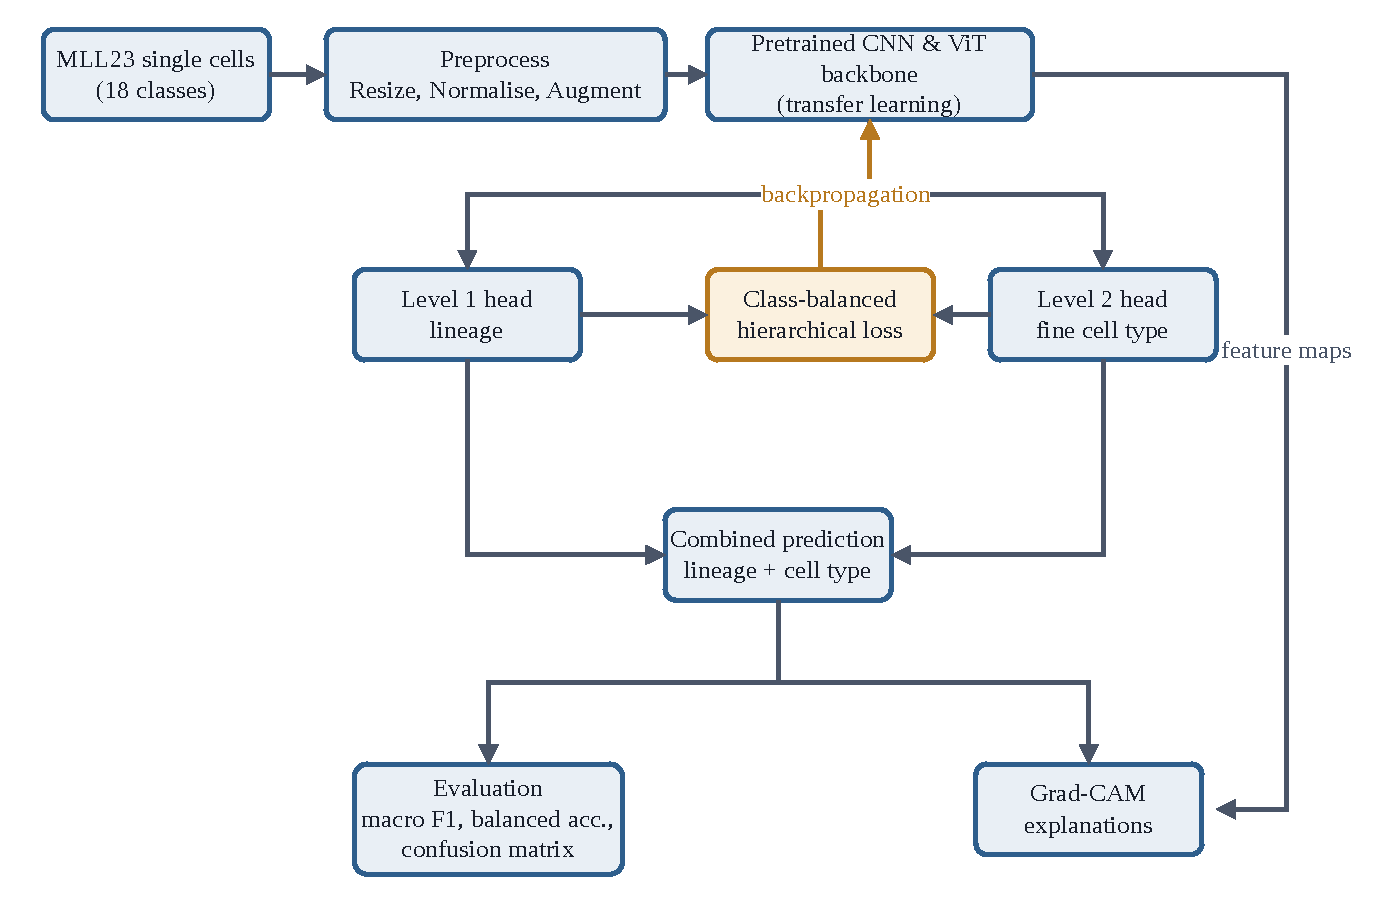
\includegraphics[width=0.86\textwidth]{Methodology-1.pdf}
  \caption{The proposed pipeline. One backbone feeds a lineage head and a fine
  cell-type head; a class-balanced hierarchical loss couples them and
  backpropagates into the shared trunk. Evaluation and Grad-CAM both read from
  the trained network.}
  \label{fig:pipeline}
\end{figure}

\section{Dataset}

\subsection{The MLL23 corpus}

The study uses the MLL23 peripheral blood single-cell dataset, published as a
data descriptor in \textit{Scientific Data} (2025) and distributed through
Zenodo under DOI \texttt{10.5281/zenodo.14277609}. It contains 41{,}621
Pappenheim-stained single nucleated-cell images at $288 \times 288$ pixels
(corresponding to a $25\,\mu\mathrm{m} \times 25\,\mu\mathrm{m}$ field), each
annotated by expert cytomorphologists into one of 18 classes.

Archives are downloaded, MD5-verified against the published checksums, and
extracted into one directory per class. A manifest is then built and the
realised per-class image counts are asserted against the counts reported in the
data descriptor. This verification is not ceremonial: a silently truncated
download or a mis-mapped class directory would corrupt every downstream result
while leaving a pipeline that still runs, and the class counts are the only
external ground truth available to detect it.

Figure~\ref{fig:examples} shows one representative image from each of the 18
classes after preprocessing. The visual difficulty of the task is apparent
directly: the myeloid maturation stages differ by gradual changes in nuclear
shape, chromatin condensation and cytoplasmic granularity rather than by any
categorical feature, and several lymphoid types are separated by subtle
differences in nuclear contour and cytoplasm volume.

\begin{figure}[H]
  \centering
  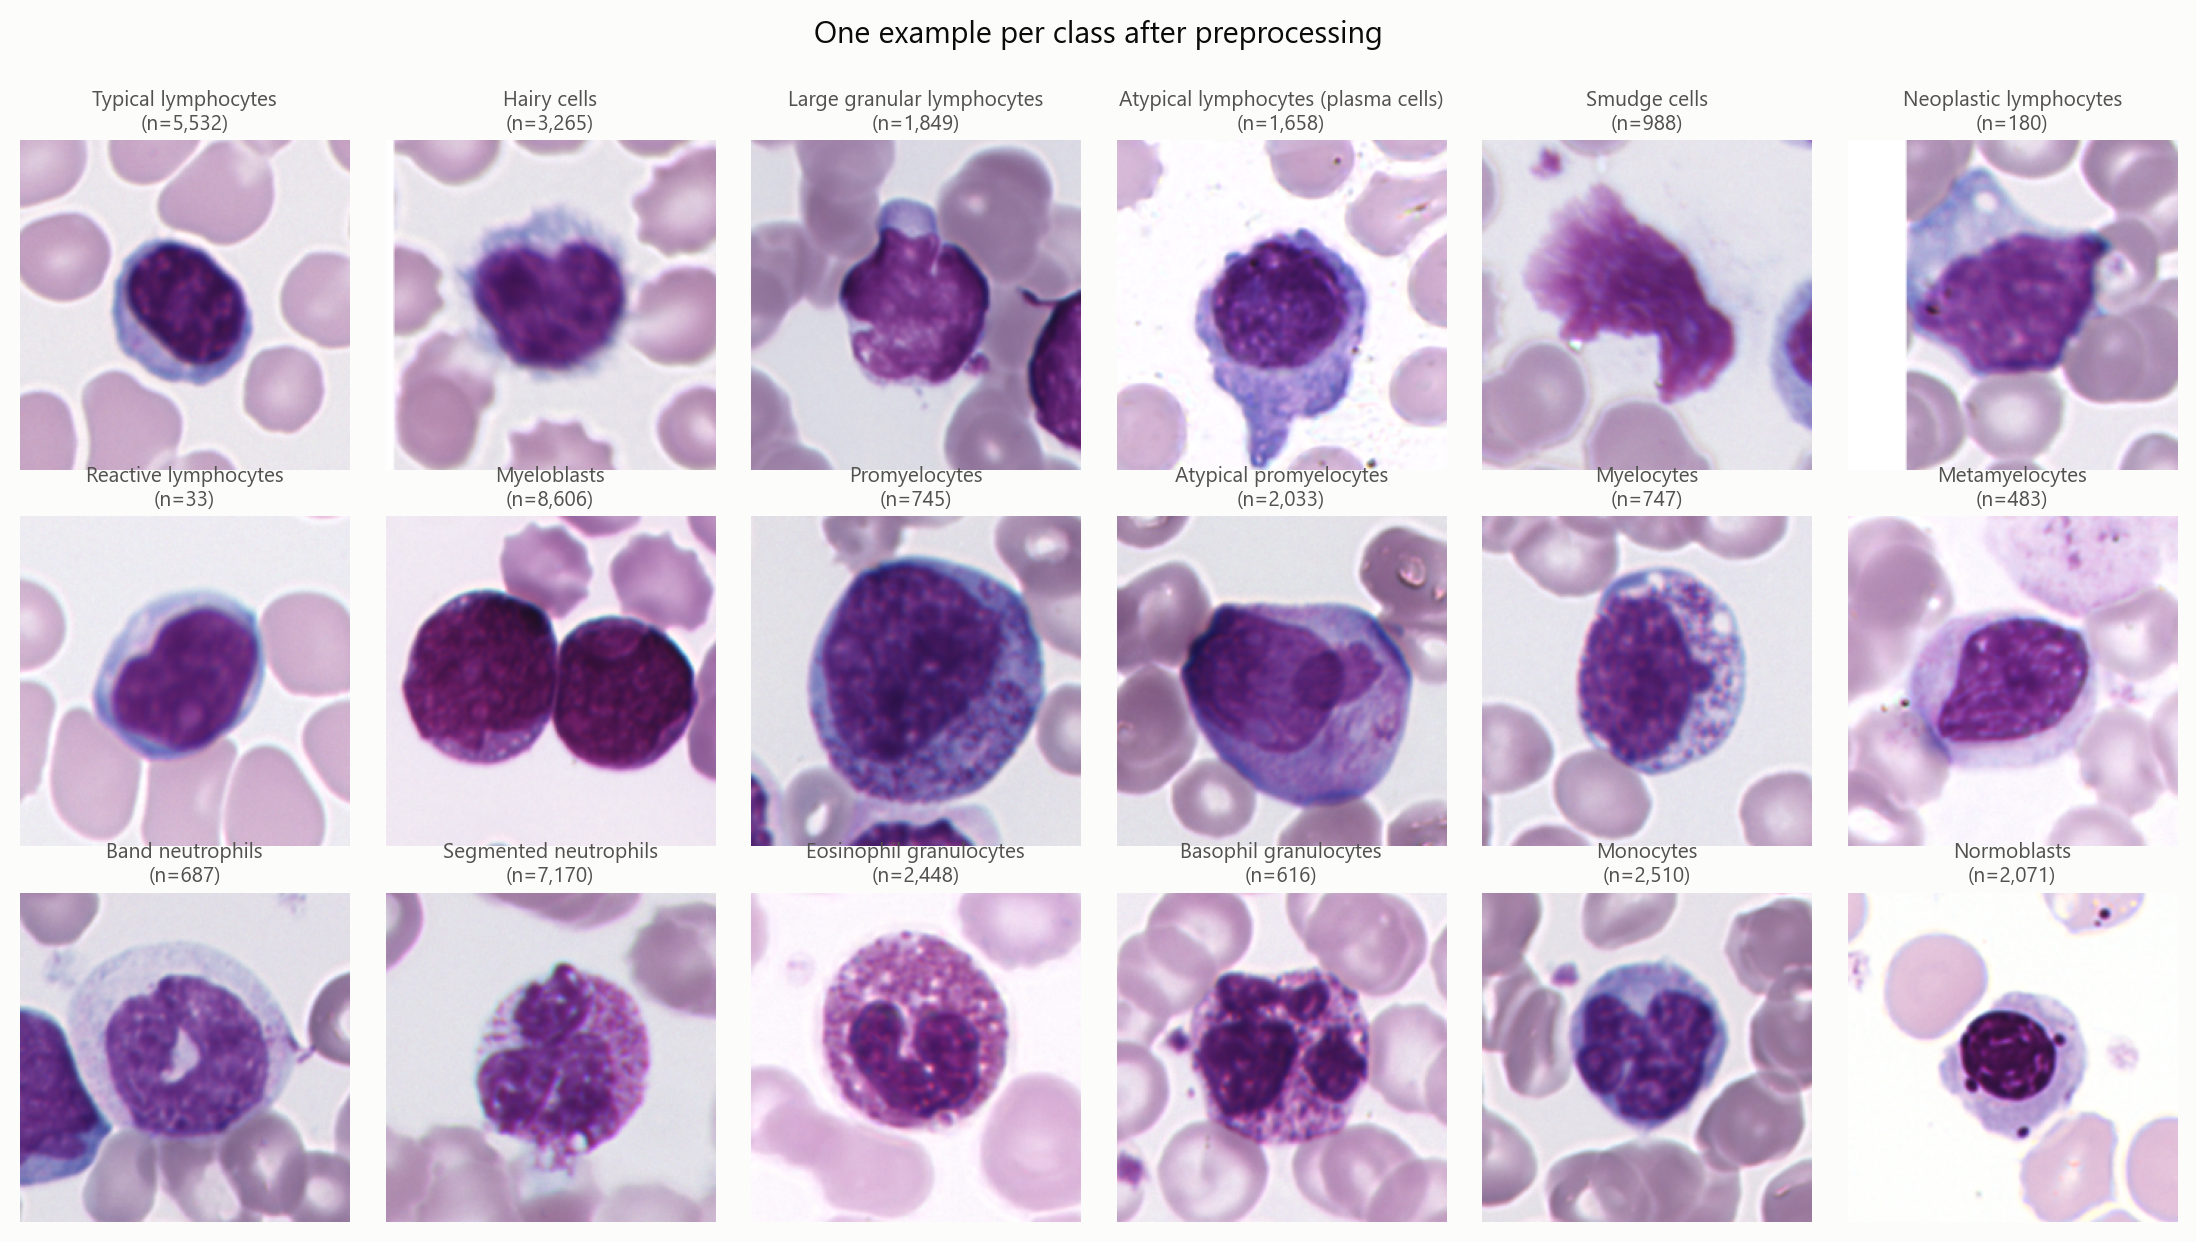
\includegraphics[width=\textwidth]{class_examples.png}
  \caption{One representative image per class after preprocessing, with corpus
  counts. Classes are shown in class-index order; within the myeloid branch this
  is the maturation continuum. The gradual morphological transition between
  adjacent stages is the source of the within-lineage confusion the study
  measures.}
  \label{fig:examples}
\end{figure}

\subsection{Label hierarchy}

Each image carries a joint target $[y_1, y_2]$, where $y_1 \in \{0,1,2\}$
denotes the haematopoietic lineage and $y_2 \in \{0,\dots,17\}$ the fine cell
type. Because every fine class belongs to exactly one lineage, the levels are
related by a fixed, non-learned surjection

\begin{equation}
  \pi : \{0,\dots,17\} \rightarrow \{0,1,2\},
  \qquad y_1 = \pi(y_2).
  \label{eq:pi}
\end{equation}

Equation~\eqref{eq:pi} is the structural prior the dissertation exploits: it is
known biology, not something the model must discover. Figure~\ref{fig:hierarchy}
gives the tree.

\begin{figure}[H]
  \centering
  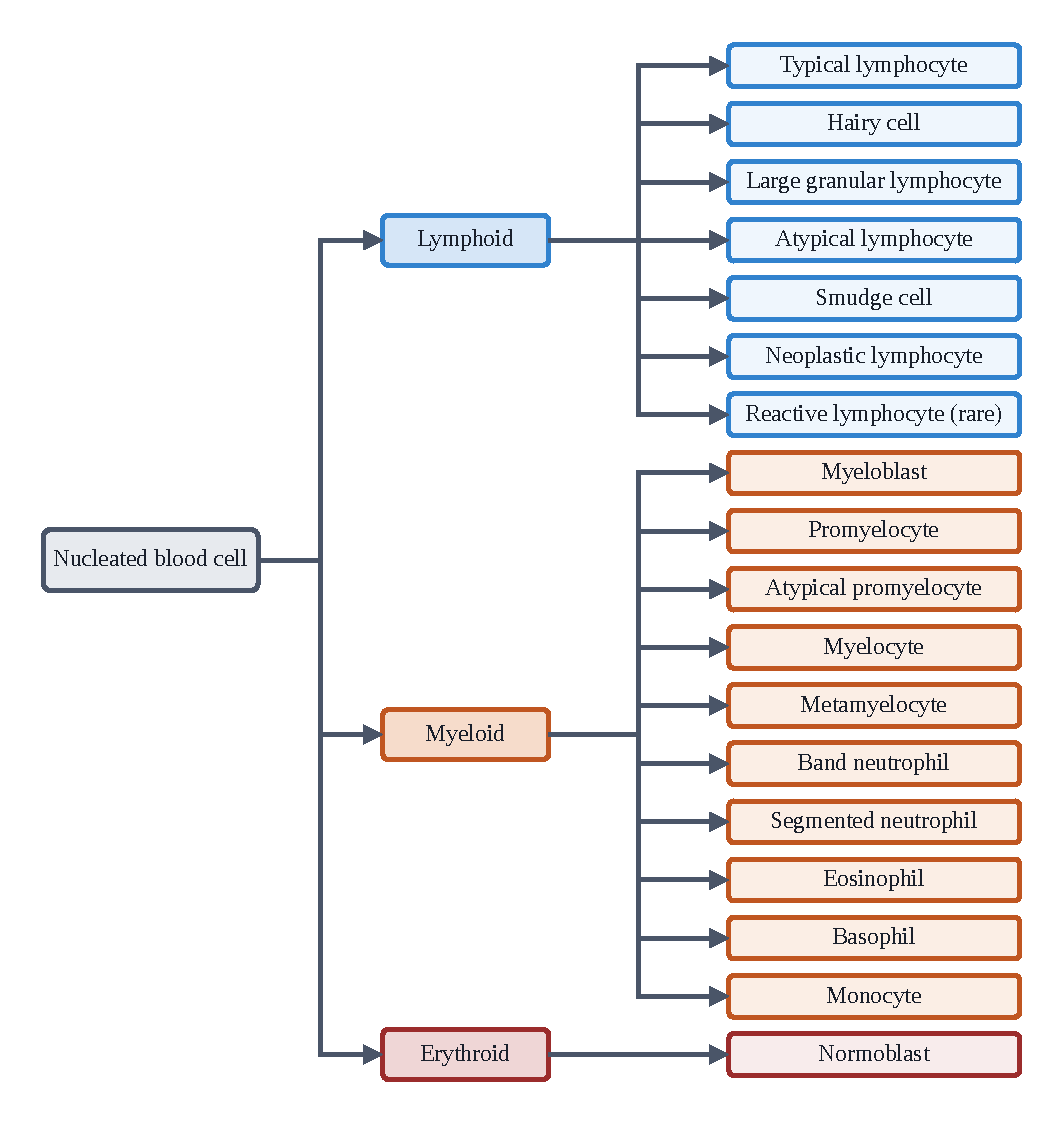
\includegraphics[width=0.92\textwidth]{cell_category.pdf}
  \caption{The two-level label hierarchy. Level~1 is the lineage; Level~2 is the
  fine cell type. Within the myeloid branch the classes follow the maturation
  continuum.}
  \label{fig:hierarchy}
\end{figure}

Fine-class indices are assigned lineage by lineage, and within the myeloid
branch they follow the maturation continuum: myeloblast $\rightarrow$
promyelocyte $\rightarrow$ myelocyte $\rightarrow$ metamyelocyte $\rightarrow$
band neutrophil $\rightarrow$ segmented neutrophil. This ordering is preserved
in the class indices and in every confusion-matrix axis, so that biologically
adjacent stages appear adjacent to the diagonal. Adjacent-stage confusion is the
clinically expected error mode, and an alphabetical or frequency-sorted axis
would scatter it across the plot and hide it.

\subsection{Class imbalance}

Table~\ref{tab:classes} reports the 18 classes with their lineage, corpus
counts, and partition sizes. Writing $n_c$ for the number of images in class
$c$, the imbalance ratio is

\begin{equation}
  \mathrm{IR} = \frac{\max_c n_c}{\min_c n_c}
              = \frac{8{,}606}{33} \approx 261.
  \label{eq:ir}
\end{equation}

Eight classes fall at or below a threshold of 1{,}000 images and are designated
\emph{minority} classes throughout. The threshold sits in a natural gap in the
distribution --- the next class above it holds 1{,}658 images --- so it
separates a genuine cluster rather than cutting one in half.
Figure~\ref{fig:dist} plots the distribution on both linear and logarithmic
axes; the logarithmic panel is the informative one, since on a linear axis the
rarest four classes are visually indistinguishable from zero.

\begin{figure}[H]
  \centering
  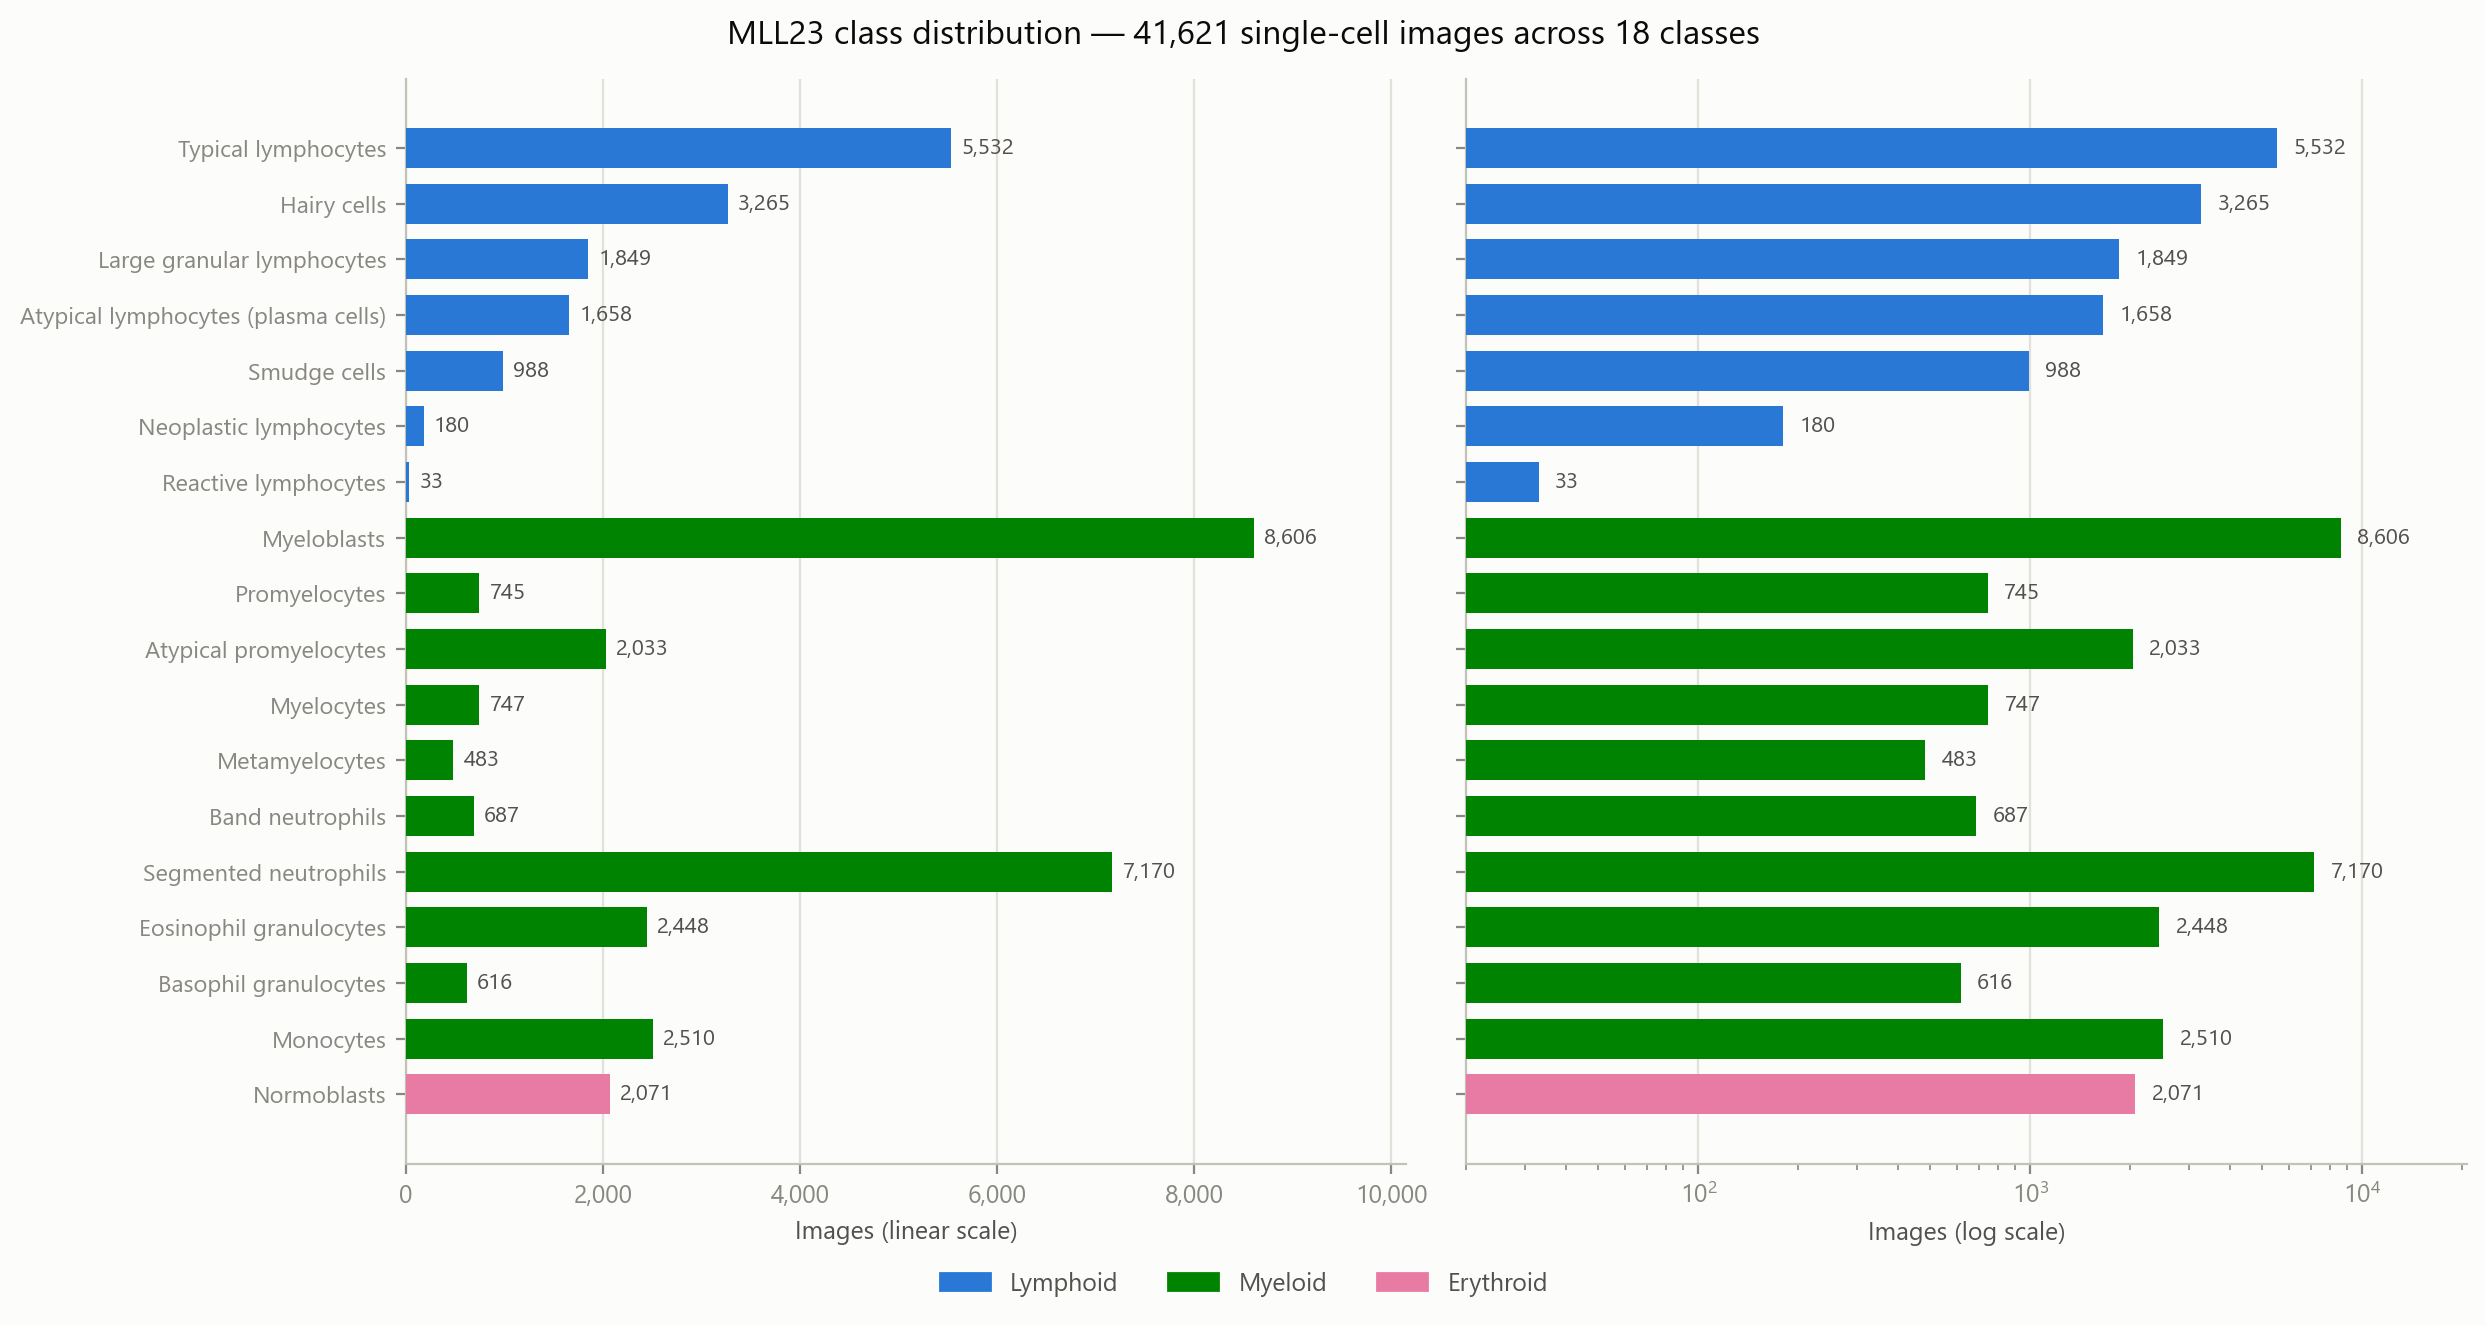
\includegraphics[width=\textwidth]{class_distribution.png}
  \caption{Class distribution on linear (left) and logarithmic (right) axes,
  coloured by lineage. The 261:1 ratio between myeloblasts and reactive
  lymphocytes is the condition the training objective must accommodate.}
  \label{fig:dist}
\end{figure}

This imbalance is the subject matter of the dissertation, not an obstacle to be
removed. It is therefore never resampled away: the training distribution is left
intact and the imbalance is addressed in the objective function
(Section~\ref{sec:loss}). Resampling would change the question being asked.

\begin{table}[H]
  \centering
  \small
  \caption{The 18 MLL23 classes, in class-index order. Minority classes
  ($n_c \le 1{,}000$) are marked $\dagger$. Partition sizes are the realised
  counts of the persisted stratified split.}
  \label{tab:classes}
  \begin{tabular}{@{}clrrrrr@{}}
    \toprule
    $y_2$ & Cell type & Total & Train & Val & Test \\
    \midrule
    \multicolumn{6}{@{}l}{\textit{Lymphoid} ($y_1 = 0$; 13,505 images)} \\
    0 & Typical lymphocytes                       & 5{,}532 & 3{,}872 & 830 & 830 \\
    1 & Hairy cells                               & 3{,}265 & 2{,}285 & 490 & 490 \\
    2 & Large granular lymphocytes                & 1{,}849 & 1{,}294 & 277 & 278 \\
    3 & Atypical lymphocytes (plasma cells)       & 1{,}658 & 1{,}161 & 249 & 248 \\
    4 & Smudge cells$^\dagger$                    &    988 &    692 & 148 & 148 \\
    5 & Neoplastic lymphocytes$^\dagger$          &    180 &    126 &  27 &  27 \\
    6 & Reactive lymphocytes$^\dagger$            &     33 &     23 &   5 &   5 \\
    \addlinespace[0.3em]
    \multicolumn{6}{@{}l}{\textit{Myeloid} ($y_1 = 1$; 26,045 images), in maturation order} \\
    7  & Myeloblasts                              & 8{,}606 & 6{,}024 & 1{,}291 & 1{,}291 \\
    8  & Promyelocytes$^\dagger$                  &    745 &    521 & 112 & 112 \\
    9  & Atypical promyelocytes                   & 2{,}033 & 1{,}423 & 305 & 305 \\
    10 & Myelocytes$^\dagger$                     &    747 &    523 & 112 & 112 \\
    11 & Metamyelocytes$^\dagger$                 &    483 &    338 &  73 &  72 \\
    12 & Band neutrophils$^\dagger$               &    687 &    481 & 103 & 103 \\
    13 & Segmented neutrophils                    & 7{,}170 & 5{,}019 & 1{,}075 & 1{,}076 \\
    14 & Eosinophil granulocytes                  & 2{,}448 & 1{,}714 & 367 & 367 \\
    15 & Basophil granulocytes$^\dagger$          &    616 &    431 &  93 &  92 \\
    16 & Monocytes                                & 2{,}510 & 1{,}757 & 376 & 377 \\
    \addlinespace[0.3em]
    \multicolumn{6}{@{}l}{\textit{Erythroid} ($y_1 = 2$; 2,071 images)} \\
    17 & Normoblasts                              & 2{,}071 & 1{,}450 & 310 & 311 \\
    \midrule
    & \textbf{Total} & \textbf{41{,}621} & \textbf{29{,}134} & \textbf{6{,}243} & \textbf{6{,}244} \\
    \bottomrule
  \end{tabular}
\end{table}

\section{Data preparation}

\subsection{Deterministic stratified partitioning}

The corpus is partitioned once into training, validation and test sets in
$70/15/15$ proportion, stratified on the fine label $y_2$. Stratifying on $y_2$
stratifies the lineage automatically, by Equation~\eqref{eq:pi}.

The partition is produced by two successive stratified draws under a fixed seed
(Algorithm~\ref{alg:split}) and then persisted to disk. Every experimental arm
reads the same persisted file, so the split is identical across arms, seeds and
backbones by construction rather than by convention.

\begin{algorithm}[H]
\caption{Deterministic stratified partitioning}
\label{alg:split}
\begin{algorithmic}[1]
\Require manifest $D$ with fine labels $y_2$; fractions $f_{\text{tr}}=0.70$,
         $f_{\text{va}}=f_{\text{te}}=0.15$; seed $s = 42$
\Ensure each row of $D$ assigned to exactly one of \{train, val, test\}
\State $(\mathcal{T}, \mathcal{H}) \gets \textproc{StratifiedSplit}(D,\ \text{train\_size}=f_{\text{tr}},\ \text{strata}=y_2,\ \text{seed}=s)$
\State $r \gets f_{\text{va}} / (1 - f_{\text{tr}})$ \Comment{share of the held-out remainder going to validation}
\State $(\mathcal{V}, \mathcal{E}) \gets \textproc{StratifiedSplit}(\mathcal{H},\ \text{train\_size}=r,\ \text{strata}=y_2[\mathcal{H}],\ \text{seed}=s)$
\State assign labels train, val, test to $\mathcal{T}, \mathcal{V}, \mathcal{E}$
\ForAll{classes $c$}
  \ForAll{partitions $P \in \{\mathcal{T}, \mathcal{V}, \mathcal{E}\}$}
    \If{$|\{i \in P : y_2^{(i)} = c\}| = 0$}
      \State \textbf{report} ``class $c$ absent from $P$'' \Comment{fails loudly rather than degrading silently}
    \EndIf
  \EndFor
\EndFor
\State \textbf{verify} no image path occurs in more than one partition
\State \textbf{verify} realised fractions deviate from requested by $< 0.01$
\State \textbf{persist} the assignment
\end{algorithmic}
\end{algorithm}

The validation loop in Algorithm~\ref{alg:split} is necessary because the rarest
class holds only 33 images. A $70/15/15$ split leaves $23/5/5$ --- thin but
non-empty in every partition, which is the guarantee the design requires. An
empty validation or test cell for that class would make its recall undefined and
silently distort the macro average, so the condition is asserted rather than
assumed.

\subsection{Preprocessing}

Evaluation preprocessing is deterministic. An image $I \in
\mathbb{Z}^{288\times288\times3}$ is bilinearly resampled to $224 \times 224$,
scaled to $[0,1]$, and standardised channel-wise:

\begin{equation}
  \hat{I}^{(k)} = \frac{I_{\downarrow}^{(k)}/255 - \mu_k}{\sigma_k},
  \qquad k \in \{R, G, B\},
  \label{eq:norm}
\end{equation}

with ImageNet statistics $\mu = (0.485, 0.456, 0.406)$ and
$\sigma = (0.229, 0.224, 0.225)$.

Two choices in Equation~\eqref{eq:norm} deserve comment. First, the input
resolution is $224 \times 224$ for \emph{every} backbone, including the Vision
Transformer. Holding resolution constant is what keeps the backbone comparison
controlled; allowing the transformer a larger input would confound architecture
with resolution. Second, ImageNet statistics are retained even though the
corpus's own channel means are $(0.742, 0.655, 0.781)$ --- brighter than
ImageNet in every channel, and widest in blue, reflecting the violet Pappenheim
stain against a bright background. After standardisation the data therefore
centres near $(1.12, 0.89, 1.67)$ rather than zero. This is intentional: the
pretrained backbones expect inputs standardised the way they were trained, and
substituting dataset-specific statistics would trade away part of the transfer
benefit. The alternative is defensible and is noted as such, but it is not the
configuration used here.

\subsection{Class-conditional augmentation}

Training applies online augmentation before the deterministic pipeline of
Equation~\eqref{eq:norm}. Augmentation is \emph{class-conditional}: minority
classes receive an intensified regime, so that the eight rarest types are
presented in greater apparent variety without altering the sampling
distribution. For a class $c$ the strength multiplier is

\begin{equation}
  s(c) = \begin{cases}
    2.0 & \text{if } n_c \le 1{,}000 \quad \text{(minority)},\\
    1.0 & \text{otherwise},
  \end{cases}
  \label{eq:augscale}
\end{equation}

applied to the rotation range and jitter magnitude, and capped as shown in
Table~\ref{tab:aug}.

\begin{table}[H]
  \centering
  \small
  \caption{Augmentation parameters. Geometric transforms are applied at the
  native 288\,px resolution, before the single downsample to 224.}
  \label{tab:aug}
  \begin{tabular}{@{}lll@{}}
    \toprule
    Transform & Majority classes & Minority classes \\
    \midrule
    Horizontal flip        & $p = 0.5$ & $p = 0.5$ \\
    Vertical flip          & $p = 0.5$ & $p = 0.5$ \\
    Random rotation        & $\pm 90^{\circ}$ & $\pm 180^{\circ}$ \\
    Brightness / contrast jitter & $0.1$ & $0.2$ \\
    RandAugment            & $2$ ops, magnitude $9$ & $3$ ops, magnitude $9$ \\
    \bottomrule
  \end{tabular}
\end{table}

Rotation is label-preserving here in a way it is not for natural images: a blood
cell has no canonical orientation, so widening the rotation range toward a full
circle adds variety without distorting the class. Rotation is performed at the
native 288\,px resolution \emph{before} the downsample, so resampling occurs once
rather than compounding, and the empty corners produced by rotating a square
frame are filled with white --- the colour of the smear background --- so that
the fill introduces no colour the network would not otherwise encounter.

An automated policy (RandAugment) is used in place of the plain jitter in the
final protocol. It replaces rather than supplements colour jitter, since
stacking two independent colour perturbations would compound them
uncontrollably. Figure~\ref{fig:aug} contrasts the three policies on a single
cell.

\begin{figure}[H]
  \centering
  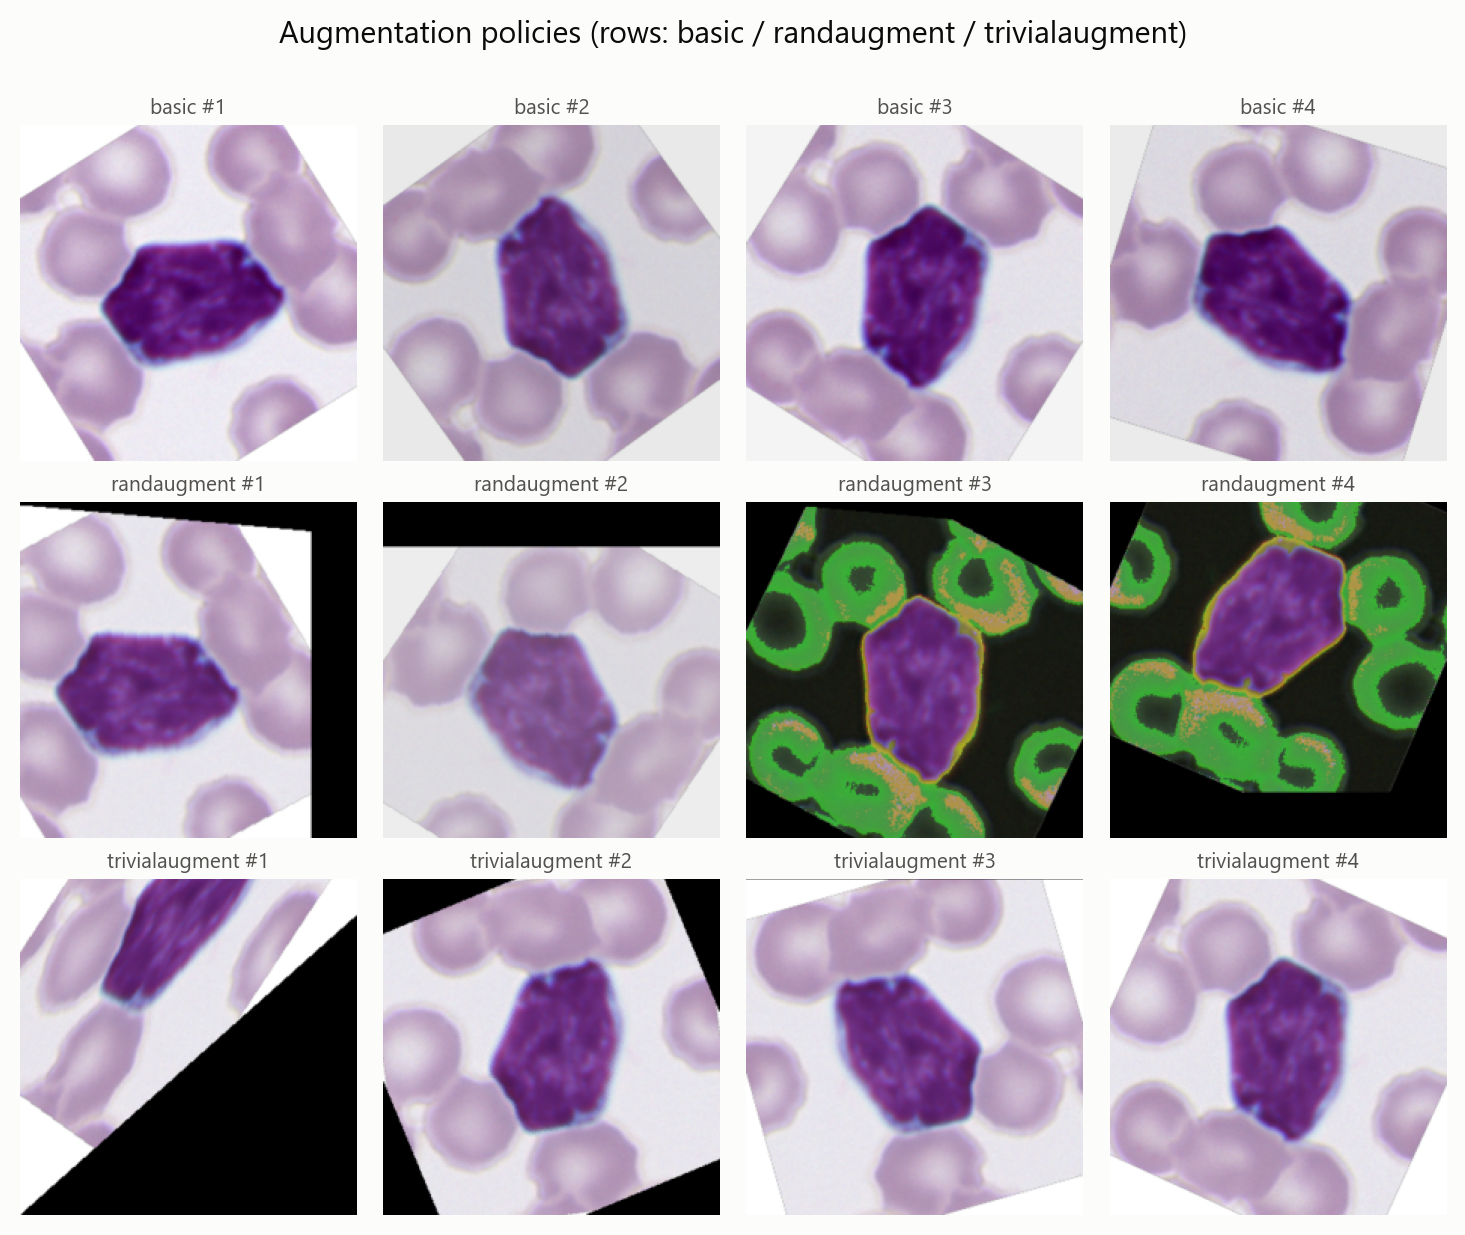
\includegraphics[width=0.86\textwidth]{augmentation_policies.png}
  \caption{The three augmentation policies applied to one image, four draws
  each. The basic policy (top) applies flips, white-filled rotation and mild
  jitter. The automated policies (middle, bottom) are markedly stronger; note
  that their internal geometric operations fill with black rather than white,
  and that RandAugment's colour operations can invert the stain palette
  entirely.}
  \label{fig:aug}
\end{figure}

Figure~\ref{fig:aug} exposes a caveat that the white-fill argument above does
not cover. The white fill is applied to the explicit rotation only; the
automated policies perform their own shear, translation and rotation
internally, and those default to a black fill. RandAugment's photometric
operations can also invert the stain palette outright, as the third and fourth
draws in the middle row show. The resulting images are far outside the
distribution of any real smear. This is a recognised property of automated
policies rather than a defect --- their regularising value comes precisely from
the severity of the perturbation, and the measured effect of enabling them was
positive --- but the ``introduces no colour the network would not otherwise
see'' justification applies strictly to the basic policy. Constraining the
automated policies to a white fill is identified as a refinement for future
work.

\subsection{Stain normalisation}

Slide preparation and imaging introduce colour variation unrelated to cell
identity. One experimental arm therefore evaluates stain normalisation as an
additional preprocessing stage, using Reinhard's method: the image is converted
to the decorrelated Lab colour space and each channel is matched to a reference
by mean and standard deviation,

\begin{equation}
  L'_k = \bigl(L_k - \bar{L}_k\bigr)\frac{\sigma_k^{\text{ref}}}{\sigma_k} + \bar{L}_k^{\text{ref}},
  \qquad k \in \{l, a, b\}.
  \label{eq:reinhard}
\end{equation}

Reinhard is preferred to Macenko for the training arm on cost grounds: Macenko
re-estimates a stain-colour basis per image from the optical-density plane and
is roughly twenty times more expensive, which at the measured data-loading
throughput would starve the GPU and make that arm slower for reasons unrelated
to the science. Macenko is retained for qualitative comparison only.

Critically, the reference statistics in Equation~\eqref{eq:reinhard} are fitted
on the \emph{training split alone}. Fitting on the full corpus would leak
validation and test colour statistics into training.

Figure~\ref{fig:stain} compares both methods against the original images.
Macenko produces the more conservative correction, preserving the relative
contrast between nucleus and cytoplasm; Reinhard shifts the overall colour
balance more aggressively, which is visible in the third row where the
background takes on a warmer cast. Whether this difference matters for
classification accuracy is an empirical question, and is precisely what the
stain-normalisation arm is designed to answer.

\begin{figure}[H]
  \centering
  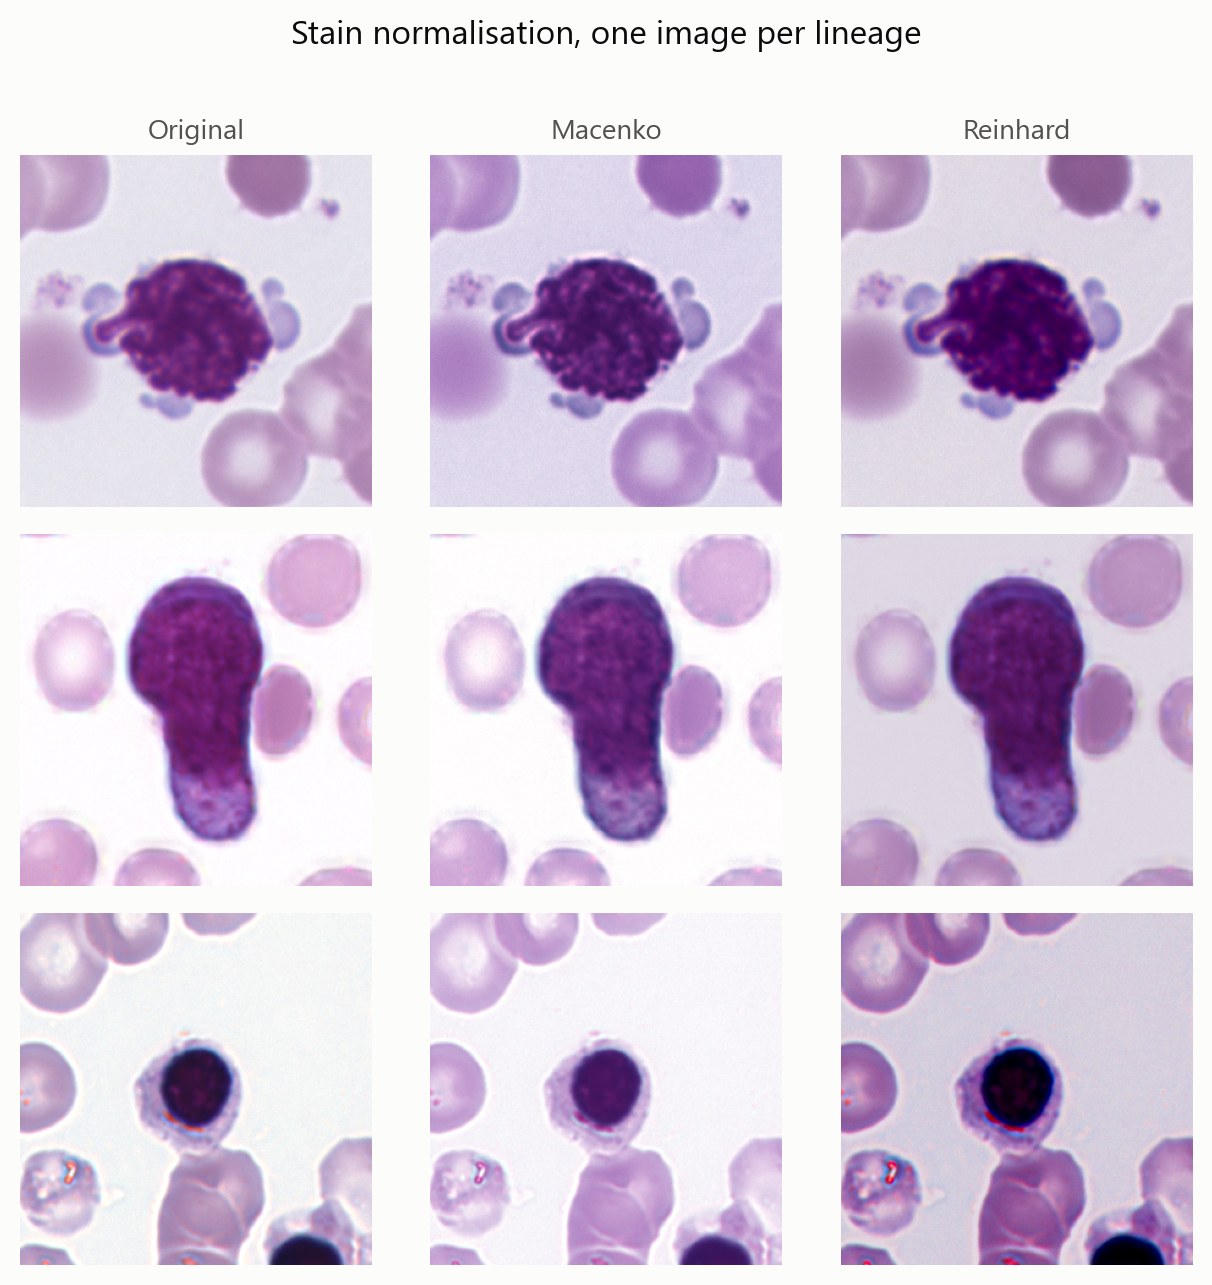
\includegraphics[width=0.56\textwidth]{stain_comparison.png}
  \caption{Stain normalisation, one image per lineage. Left: original. Centre:
  Macenko, which re-estimates a stain-colour basis per image. Right: Reinhard,
  which matches channel statistics in Lab space and is the method used in the
  training arm on cost grounds.}
  \label{fig:stain}
\end{figure}

\subsection{Decoded-image cache}

Throughput measurement showed the pipeline to be data-bound rather than
compute-bound: decoding TIFFs sustained 178 images/s at four workers, and
\emph{fell} to 119 images/s at eight from worker contention, against a
full training step of 82 images/s. Decoding was therefore the binding
constraint, and backbone choice barely moved wall-clock time.

A cache of decoded images at native $288$\,px resolution raises throughput to
approximately 850 images/s. Caching at 288 rather than at the model input size
is deliberate: it preserves the property that rotation precedes the single
downsample, so the cache removes decode cost without altering augmentation
semantics. A separate cache holds the Reinhard-normalised variant, so that the
stain arm runs at the same throughput as the others and a runtime difference
between arms never becomes a confound.

\section{Model architecture}

\subsection{Shared backbone with two heads}

The model is a pretrained backbone $f_\theta$ producing a pooled $D$-dimensional
representation, followed by two linear heads:

\begin{align}
  z &= \mathrm{Dropout}\bigl(f_\theta(\hat{I})\bigr), \qquad z \in \mathbb{R}^{D}, \label{eq:trunk}\\
  \mathbf{u} &= W_1 z + b_1, \qquad \mathbf{u} \in \mathbb{R}^{3} \quad \text{(lineage logits)}, \label{eq:head1}\\
  \mathbf{v} &= W_2 z + b_2, \qquad \mathbf{v} \in \mathbb{R}^{18} \quad \text{(fine logits)}. \label{eq:head2}
\end{align}

The two heads are trained jointly on the shared trunk, so the coarse decision
regularises the fine one and rare types borrow representational strength from
their lineage neighbours. Figure~\ref{fig:arch} shows the coupling.

\begin{figure}[H]
\centering
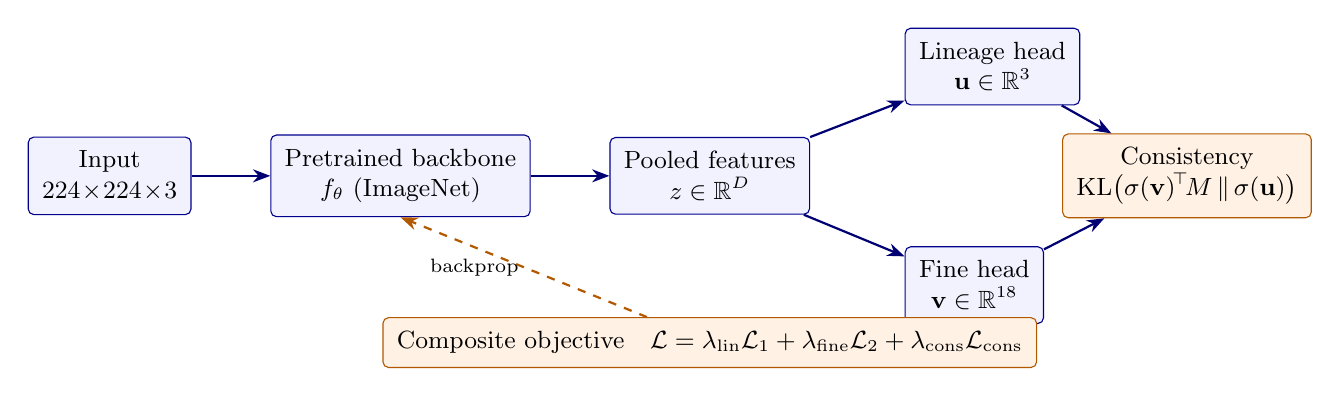
\begin{tikzpicture}[
  node distance=6mm,
  box/.style={draw=blue!55!black, fill=blue!5, rounded corners=2pt,
              align=center, inner sep=5pt, font=\small},
  lossbox/.style={draw=orange!70!black, fill=orange!10, rounded corners=2pt,
              align=center, inner sep=5pt, font=\small},
  ar/.style={-{Stealth[length=2.2mm]}, draw=blue!45!black, thick},
  arg/.style={-{Stealth[length=2.2mm]}, draw=orange!70!black, thick, dashed},
  lbl/.style={font=\scriptsize, inner sep=1.5pt}
]
\node[box] (img) {Input\\$224\!\times\!224\!\times\!3$};
\node[box, right=10mm of img] (bb) {Pretrained backbone\\$f_\theta$ (ImageNet)};
\node[box, right=10mm of bb] (z) {Pooled features\\$z \in \mathbb{R}^{D}$};

\node[box, above right=4mm and 12mm of z] (h1) {Lineage head\\$\mathbf{u} \in \mathbb{R}^{3}$};
\node[box, below right=4mm and 12mm of z] (h2) {Fine head\\$\mathbf{v} \in \mathbb{R}^{18}$};

\node[lossbox, right=32mm of z] (cons) {Consistency\\$\mathrm{KL}\bigl(\sigma(\mathbf{v})^{\!\top}\!M \,\|\, \sigma(\mathbf{u})\bigr)$};

\draw[ar] (img) -- (bb);
\draw[ar] (bb) -- (z);
\draw[ar] (z) -- (h1);
\draw[ar] (z) -- (h2);
\draw[ar] (h1) -- (cons);
\draw[ar] (h2) -- (cons);

\node[lossbox, below=13mm of z] (loss)
  {Composite objective\quad
   $\mathcal{L} = \lambda_{\text{lin}}\mathcal{L}_1 + \lambda_{\text{fine}}\mathcal{L}_2 + \lambda_{\text{cons}}\mathcal{L}_{\text{cons}}$};
\draw[arg] (loss) -- node[lbl, left] {backprop} (bb.south);
\end{tikzpicture}
\caption{The two-head architecture. Both heads read the same pooled
representation; the consistency term marginalises the fine posterior into
lineage space through the fixed map $M$ and penalises disagreement with the
lineage head. Gradients from all three terms flow into the shared backbone.}
\label{fig:arch}
\end{figure}

A single class implements every arm. In hierarchical mode both heads are
constructed and returned; in flat mode the lineage head is never constructed, so
it contributes neither parameters nor weight decay --- an unused head would make
the ``identical backbone'' claim quietly false. At inference the flat model's
lineage prediction is derived from its fine prediction through
Equation~\eqref{eq:pi}, which is what makes the hierarchical error decomposition
of Section~\ref{sec:hierrors} computable for the baseline and hence comparable
across arms.

\subsection{Why the lineage head regularises rather than gates}

An obvious alternative architecture is a hard gate: predict the lineage first,
then route the sample to one of three per-lineage sub-classifiers. That design
was considered and rejected on evidence. Exploratory analysis on frozen ImageNet
features measured a lineage silhouette coefficient of approximately zero --- the
lineages do \emph{not} form separable global clusters --- while $k$-nearest-neighbour
lineage agreement was approximately $0.78$ against a chance baseline of $0.45$.
The lineage structure is therefore real but \emph{local}.

A hard gate assumes global separability, which the data rejects, and every gate
misfire would produce an unrecoverable cross-lineage error. The soft coupling
used instead --- a shared trunk plus a consistency penalty --- exploits the local
structure that exists without asserting the global structure that does not.
Figure~\ref{fig:umap} shows the evidence.

\begin{figure}[H]
  \centering
  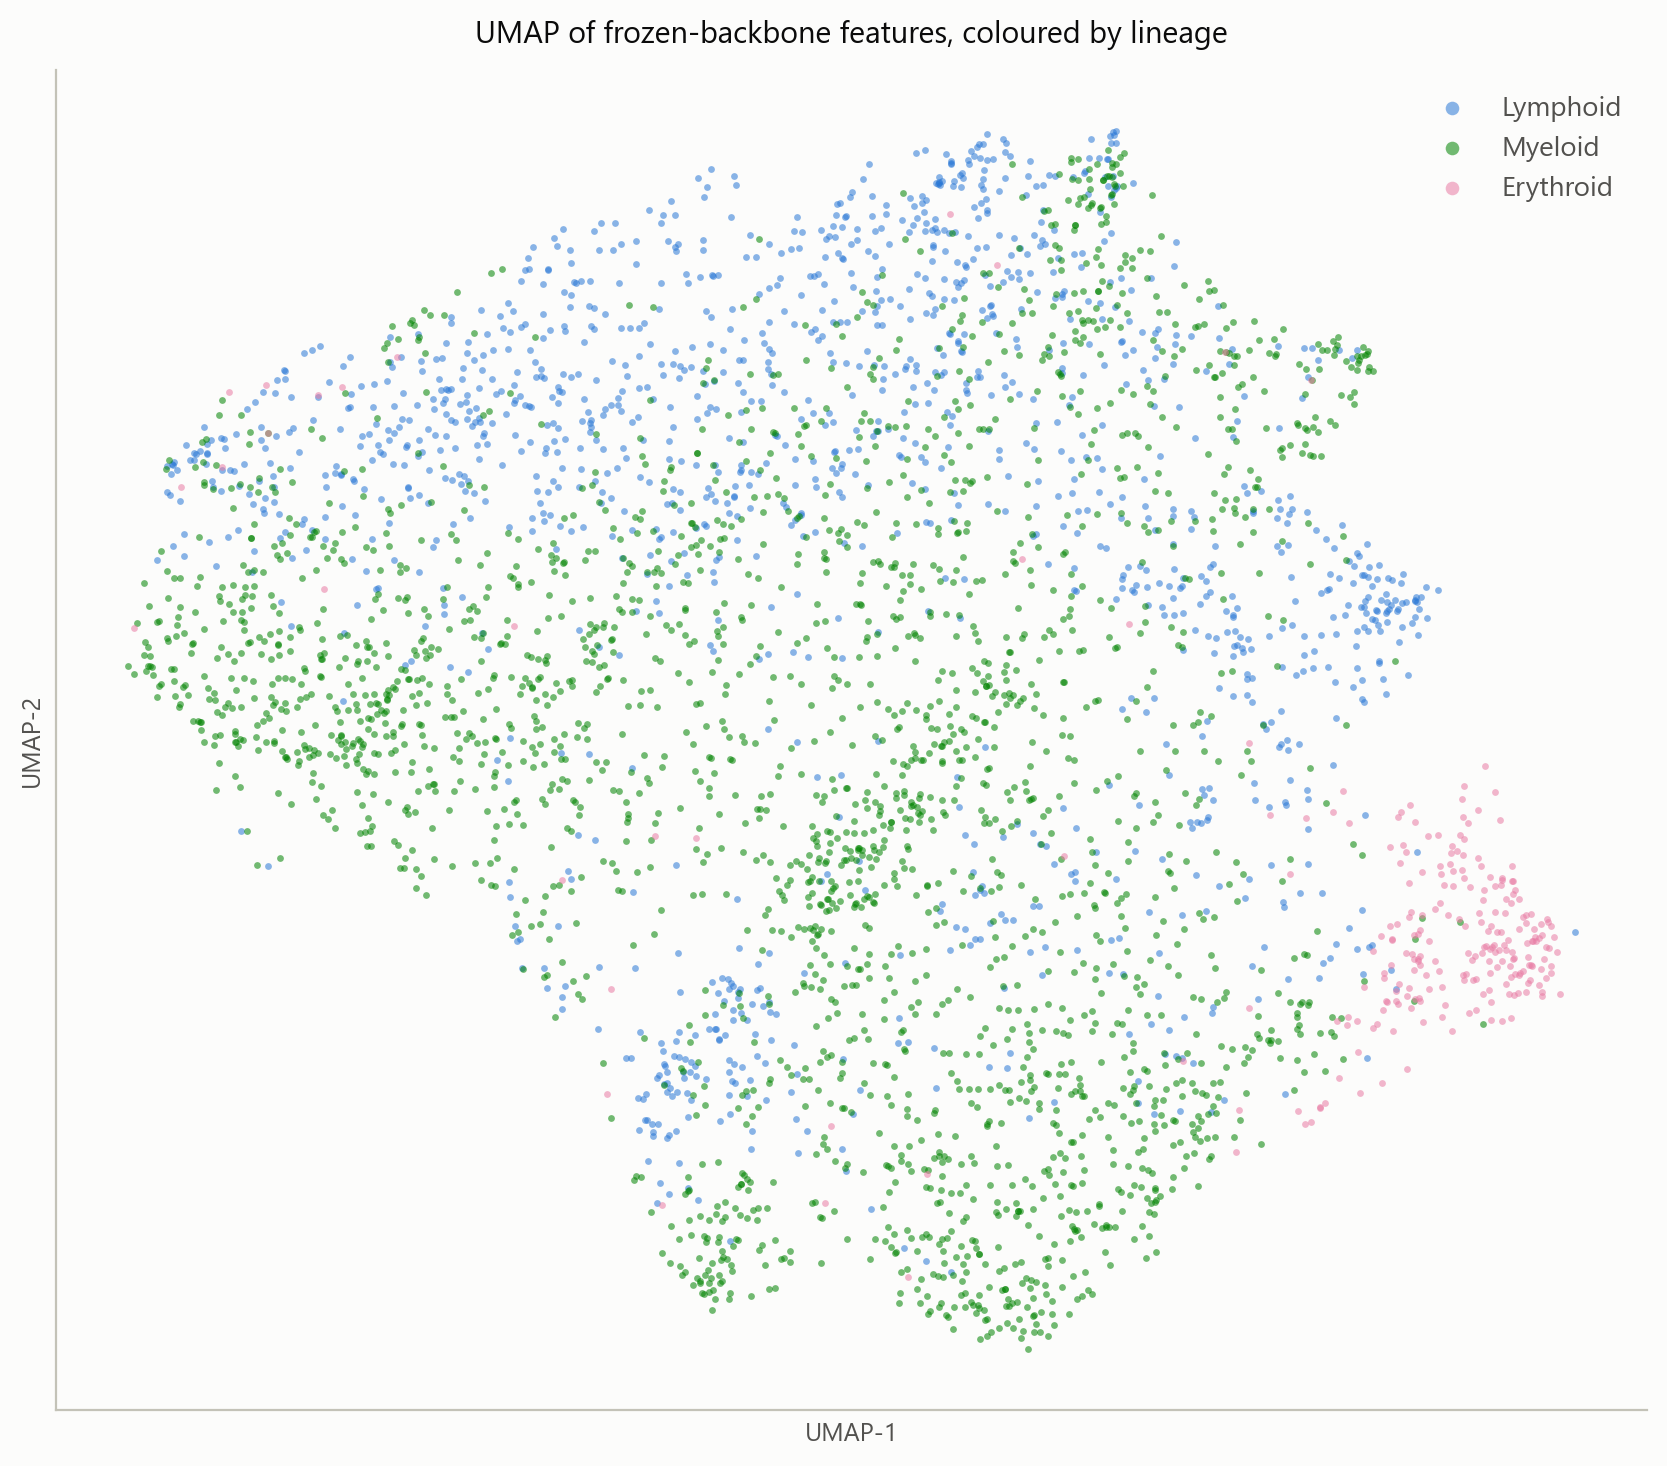
\includegraphics[width=0.66\textwidth]{umap_lineage.png}
  \caption{UMAP projection of frozen ImageNet backbone features, coloured by
  lineage. The lineages interleave rather than forming separable clusters,
  which is what rules out a hard routing gate. The structure that does exist is
  local: a cell's nearest neighbours usually share its lineage even though the
  lineages form no global cluster.}
  \label{fig:umap}
\end{figure}

Two caveats attach to Figure~\ref{fig:umap}. It is a two-dimensional projection,
so apparent overlap is weaker evidence than the silhouette coefficient quoted
above; and it is computed on \emph{frozen} features, before any fine-tuning.
Fine-tuning may well induce more lineage separation than the projection shows.
The figure motivates the architectural choice; it does not by itself establish
the limits of what the trained model can represent.

\subsection{Candidate backbones}

Four backbones are compared (Table~\ref{tab:backbones}), spanning a lightweight
CNN, a standard residual CNN, a modernised CNN, and a transformer. All are
initialised from ImageNet weights and fully fine-tuned. The head input width is
measured with a single dummy forward pass at construction rather than read from
the library's reported feature count, which is unreliable for some
architectures.

\begin{table}[H]
  \centering
  \small
  \caption{Candidate backbones. All are fine-tuned end to end at
  $224 \times 224$.}
  \label{tab:backbones}
  \begin{tabular}{@{}lll@{}}
    \toprule
    Key & Architecture & Family \\
    \midrule
    \texttt{mobilenet} & MobileNetV3-Large & Lightweight CNN \\
    \texttt{resnet}    & ResNet-50         & Residual CNN \\
    \texttt{convnext}  & ConvNeXt-Tiny     & Modernised CNN \\
    \texttt{vit}       & ViT-Small/16      & Vision Transformer \\
    \bottomrule
  \end{tabular}
\end{table}

\section{Training objective}
\label{sec:loss}

The objective has three components. Two address imbalance; the third couples the
label levels.

\subsection{Class-balanced weighting}

Samples of the same class overlap in feature space, so the $n$-th sample of a
class contributes less new information than the first. Following Cui et al., the
\emph{effective number} of samples of a class with $n_c$ images is
$(1 - \beta^{n_c})/(1 - \beta)$, and the class weight is its reciprocal:

\begin{equation}
  w_c = \frac{1 - \beta}{1 - \beta^{n_c}},
  \qquad
  \tilde{w}_c = \frac{w_c}{\frac{1}{C}\sum_{j} w_j},
  \qquad \beta = 0.9999.
  \label{eq:cb}
\end{equation}

As $\beta \rightarrow 0$ this recovers uniform weighting; as $\beta \rightarrow 1$
it approaches inverse-frequency weighting. The normalisation to unit mean in
Equation~\eqref{eq:cb} is essential to the ablation design: without it, the
weighted arm would train at a different effective learning rate and the
comparison would confound reweighting with step size. The same construction is
applied at the lineage level, where the counts are the sums over each lineage's
members --- the lineage level is itself imbalanced, myeloid accounting for
roughly 63\% of the corpus.

\subsection{Focal loss}

Class weighting addresses \emph{how many} samples a class has; it does not
address \emph{how hard} an individual sample is. The focal loss of Lin et al.
supplies the second factor, down-weighting confidently correct examples so that
the gradient is not dominated by the 8{,}606 myeloblasts:

\begin{equation}
  \mathcal{L}_{\text{focal}}(\mathbf{v}, y)
    = \bigl(1 - p_y\bigr)^{\gamma}\,
      \mathrm{CE}\bigl(\mathbf{v}, y;\ \tilde{w}\bigr),
  \qquad
  p_y = \mathrm{softmax}(\mathbf{v})_y,
  \qquad \gamma = 2.
  \label{eq:focal}
\end{equation}

The modulating factor $p_y$ in Equation~\eqref{eq:focal} is computed from the
\emph{unweighted} posterior. It should reflect the difficulty of the sample, not
the rarity of its class; the class weight $\tilde{w}$ already carries rarity, and
folding it into both factors would double-count it.

\subsection{Hierarchical consistency}

The term that makes the objective hierarchical rather than merely multi-task
couples the two heads. Let $M \in \{0,1\}^{18 \times 3}$ be the one-hot matrix
of the map $\pi$ from Equation~\eqref{eq:pi}. Right-multiplying a fine posterior
by $M$ marginalises it into lineage space, since each fine class belongs to
exactly one lineage. The consistency penalty is the Kullback--Leibler divergence
between that marginalised belief and the lineage head's own posterior:

\begin{equation}
  \mathcal{L}_{\text{cons}}
    = \mathrm{KL}\Bigl(
        \mathrm{softmax}(\mathbf{v})^{\top} M
        \,\Bigl\|\,
        \mathrm{softmax}(\mathbf{u})
      \Bigr).
  \label{eq:cons}
\end{equation}

Without Equation~\eqref{eq:cons} the two heads are free to contradict each other
and the claim that the coarse decision regularises the fine one has no mechanism
behind it. Gradients flow into both heads, pulling them toward agreement rather
than forcing one to chase the other.

\subsection{Composite objective and ablation switches}

The three components combine as

\begin{equation}
  \mathcal{L} = \lambda_{\text{lin}}\,\mathcal{L}_{\text{focal}}(\mathbf{u}, y_1)
              + \lambda_{\text{fine}}\,\mathcal{L}_{\text{focal}}(\mathbf{v}, y_2)
              + \lambda_{\text{cons}}\,\mathcal{L}_{\text{cons}},
  \label{eq:total}
\end{equation}

with $\lambda_{\text{lin}} = 0.3$, $\lambda_{\text{fine}} = 1.0$ and
$\lambda_{\text{cons}} = 0.1$. The fine term is held at unity because it is the
task being evaluated. The consistency weight is deliberately small, for the
reason given above: the empirical support is for \emph{local} lineage structure,
so consistency is applied as a nudge and not as a constraint. Forcing it hard
would impose a global structure the data does not exhibit.

The two ablations are field values on this one object rather than separate loss
classes (Table~\ref{tab:ablation}), which is what keeps the arms honest.

\begin{table}[H]
  \centering
  \small
  \caption{The ablation switches. Both are implemented as parameters of a single
  loss object, not as alternative implementations.}
  \label{tab:ablation}
  \begin{tabular}{@{}lll@{}}
    \toprule
    Switch & Effect & Purpose \\
    \midrule
    \texttt{use\_hierarchy = False}
      & $\lambda_{\text{lin}} = \lambda_{\text{cons}} = 0$
      & Fine-level loss only; removes the hierarchy \\
    \texttt{use\_imbalance = False}
      & $\tilde{w} \equiv 1,\ \gamma = 0$, no smoothing
      & Plain cross-entropy; removes the imbalance treatment \\
    \bottomrule
  \end{tabular}
\end{table}

\subsection{Hierarchical mixing}

MixUp and CutMix blend two examples and their labels. Because MLL23 carries two
label levels, a mix must remain consistent across levels: the same coefficient
$\lambda$ applies to both targets, so the coarse and fine losses see the same
blend. Applying independent mixes per level would let the objective disagree with
itself about how much of each example is present. For a batch and a shuffled
partner indexed by permutation $\rho$,

\begin{equation}
  \tilde{x} = \lambda x + (1-\lambda)\,x_{\rho},
  \qquad
  \mathcal{L} = \lambda\,\mathcal{L}(\cdot,\, y) + (1-\lambda)\,\mathcal{L}(\cdot,\, y_{\rho}),
  \qquad \lambda \sim \mathrm{Beta}(\alpha, \alpha).
  \label{eq:mix}
\end{equation}

Labels are interpolated in the \emph{loss} rather than mixed as hard targets,
which keeps the class-balanced weighting of Equation~\eqref{eq:cb} well defined.
For CutMix, $\lambda$ is recomputed from the realised patch area, since integer
pixel boundaries rarely match the sampled ratio exactly.

\section{Training protocol}

\subsection{Optimisation}

Training uses AdamW with decoupled weight decay, a linear warmup over the first
epoch, and cosine annealing thereafter over a \emph{fixed} budget of $T$ total
steps:

\begin{equation}
  \eta_t = \begin{cases}
    \eta_0 \dfrac{t+1}{T_{\text{w}}}, & t < T_{\text{w}},\\[2ex]
    \dfrac{\eta_0}{2}\left(1 + \cos\pi\dfrac{t - T_{\text{w}}}{T - T_{\text{w}}}\right), & t \ge T_{\text{w}}.
  \end{cases}
  \label{eq:lr}
\end{equation}

Warmup matters with pretrained weights: a full-magnitude step into an ImageNet
initialisation at the start of training discards much of what transfer learning
provides.

Early stopping is disabled, and this is a deliberate correction. The cosine
schedule of Equation~\eqref{eq:lr} is defined over the configured budget, so
stopping early truncates the anneal and leaves the model mid-training at a high
learning rate. An earlier iteration of this study configured 50 epochs but
stopped between 12 and 37, leaving runs at up to 86\% of peak learning rate; the
number of epochs a run survived then correlated with its score at $r = +0.87$,
so the arm ranking largely measured the stopping rule rather than the method. A
fixed budget guarantees every arm receives an identical anneal.

\subsection{Variance reduction}

Two mechanisms reduce the noise in the quantity used for model selection. An
exponential moving average of the weights is maintained,

\begin{equation}
  \theta^{\text{EMA}}_t = d\,\theta^{\text{EMA}}_{t-1} + (1-d)\,\theta_t,
  \qquad d = 0.999,
  \label{eq:ema}
\end{equation}

and the averaged weights --- not the live ones --- are evaluated, selected and
reported. At test time, predictions are averaged over the four horizontal and
vertical flip combinations; since blood cells have no canonical orientation,
these are genuine label-preserving equivalents rather than distortions.

The justification is measured. Raw epoch-to-epoch validation macro F1 varies with
standard deviation $0.021$, which is \emph{larger} than the between-arm
differences under study. Without smoothing, checkpoint selection would be closer
to a lottery than a decision. Together these mechanisms reduce that variation to
$0.0097$, a 54\% reduction.

\subsection{Numerical precision}

Mixed precision uses bfloat16 rather than float16. A float16 run reached
validation macro F1 of $0.80$ and then diverged to NaN at the third epoch,
wasting the remainder of the run --- NaN weights never recover. bfloat16 retains
float32's exponent range and so cannot overflow in the same way. Gradient
scaling, which exists to prevent float16 gradient underflow, is correspondingly
disabled. The loss itself is computed in float32 regardless of the surrounding
autocast context, because the class-balanced weights span a wide range and the
focal term exponentiates a log-probability; both are numerically delicate in
reduced precision.

\subsection{The training loop}

Table~\ref{tab:hyper} lists the hyperparameters, which are held identical across
every arm. Algorithm~\ref{alg:train} states one training run. Model selection is
on validation macro F1 and never on accuracy: at an imbalance ratio of 261, a
classifier that ignores reactive lymphocytes entirely forfeits under $0.1\%$ of
accuracy, so an accuracy-selected checkpoint is precisely one that has learned to
abandon the classes the study is about.

\begin{algorithm}[H]
\caption{One training run}
\label{alg:train}
\begin{algorithmic}[1]
\Require configuration $\kappa$; persisted split; training class counts $n$
\Ensure checkpoint selected on best validation macro F1
\State seed Python, NumPy and Torch from $\kappa.\text{seed}$
\State build model in mode $\kappa.\text{mode}$; build $\mathcal{L}$ from $n$, $\kappa.\text{use\_hierarchy}$, $\kappa.\text{use\_imbalance}$
\State $\theta^{\text{EMA}} \gets \theta$;\quad $F^{\star} \gets -\infty$
\For{epoch $= 1$ to $\kappa.\text{epochs}$}
  \ForAll{batches $(x, y_1, y_2)$}
    \State $(\tilde{x}, y_a, y_b, \lambda) \gets \textproc{MaybeMix}(x, y_1, y_2)$ \Comment{one $\lambda$ shared by both levels}
    \State $(\mathbf{u}, \mathbf{v}) \gets$ forward pass under bfloat16 autocast
    \State $\ell \gets \lambda\,\mathcal{L}(\cdot, y_a) + (1-\lambda)\,\mathcal{L}(\cdot, y_b)$ \Comment{computed in float32}
    \If{$\ell$ is not finite}
      \State \textbf{skip} the optimiser step \Comment{never propagate NaN into the weights}
    \Else
      \State backpropagate; step AdamW; step the schedule of Eq.~\eqref{eq:lr}
      \State update $\theta^{\text{EMA}}$ by Eq.~\eqref{eq:ema}
    \EndIf
  \EndFor
  \State $F \gets$ validation macro F1 of $\theta^{\text{EMA}}$
  \If{$F > F^{\star}$} \State $F^{\star} \gets F$; checkpoint $\theta^{\text{EMA}}$ \EndIf
  \State append epoch metrics to the run history
\EndFor
\State \textbf{evaluate} the selected checkpoint on the test split with 4-view TTA
\end{algorithmic}
\end{algorithm}

\begin{table}[H]
  \centering
  \small
  \caption{Training hyperparameters, held identical across all arms.}
  \label{tab:hyper}
  \begin{tabular}{@{}ll@{}}
    \toprule
    Parameter & Value \\
    \midrule
    Optimiser                 & AdamW \\
    Learning rate $\eta_0$    & $3 \times 10^{-4}$ \\
    Weight decay              & $0.05$ \\
    Batch size                & 64 \\
    Epochs                    & 30 (fixed; no early stopping) \\
    Warmup                    & 1 epoch, linear \\
    Schedule                  & Cosine annealing \\
    Label smoothing           & $0.05$ \\
    Focal $\gamma$            & $2.0$ \\
    Class-balanced $\beta$    & $0.9999$ \\
    Loss weights              & $\lambda_{\text{lin}}=0.3$, $\lambda_{\text{fine}}=1.0$, $\lambda_{\text{cons}}=0.1$ \\
    Augmentation policy       & RandAugment (class-conditional) \\
    Batch mixing              & CutMix, $p = 0.5$, $\alpha = 1.0$ \\
    Weight EMA decay          & $0.999$ \\
    Test-time augmentation    & 4 flip views \\
    Mixed precision           & bfloat16 \\
    Model selection           & Validation macro F1 \\
    \bottomrule
  \end{tabular}
\end{table}

\section{Experimental design}

\subsection{The arms}

Five experiments are required, under identical splits and backbones. They reduce
to four distinct configurations (Table~\ref{tab:arms}), because the hierarchy
ablation applied to the proposed model \emph{is} the flat baseline: removing the
lineage head and its loss terms from the two-head model leaves a single-head
18-class classifier. That configuration is trained once and reported twice. The
alternative --- training the identical configuration under two names --- would
consume a fifth of the compute budget to produce two draws from the same
distribution and invite the reader to mistake them for independent evidence.

\begin{table}[H]
  \centering
  \small
  \caption{The four distinct configurations and the five reported experiments.}
  \label{tab:arms}
  \begin{tabular}{@{}llcccl@{}}
    \toprule
    Arm & Mode & Hierarchy & Imbalance & Stain & Reported as \\
    \midrule
    \texttt{flat\_baseline} & flat & --- & \checkmark & --- & 1. Flat baseline; 4. Hierarchy ablation \\
    \texttt{hierarchical}   & hier & \checkmark & \checkmark & --- & 2. Full hierarchical model (proposed) \\
    \texttt{no\_imbalance}  & hier & \checkmark & --- & --- & 3. Imbalance ablation \\
    \texttt{stain\_norm}    & hier & \checkmark & \checkmark & \checkmark & 5. Stain-normalised input \\
    \bottomrule
  \end{tabular}
\end{table}

\subsection{Two phases}

Phase~1 screens the four backbones of Table~\ref{tab:backbones} under the
hierarchical configuration for a short fixed budget at one seed, and selects the
backbone carried into Phase~2 on validation macro F1. This is a
\emph{selection} run and not the backbone comparison result: a short budget need
not rank backbones the way a full run would, and the write-up states this as a
limitation rather than presenting the screen as evidence.

Phase~2 trains the four configurations of Table~\ref{tab:arms} at three seeds
each on the selected backbone, giving twelve runs. The matrix is resumable: a run
already recorded in the results file is skipped, so an interruption costs only
the unfinished runs.

\section{Evaluation}

\subsection{Metrics}

Plain accuracy is explicitly rejected as a headline number. At an imbalance ratio
of 261 it cannot see the behaviour under study. The headline metrics are macro F1
and balanced accuracy, which weight every class equally regardless of frequency:

\begin{equation}
  \text{macro-}F_1 = \frac{1}{C}\sum_{c=1}^{C}
    \frac{2\,P_c R_c}{P_c + R_c},
  \qquad
  \text{balanced accuracy} = \frac{1}{C}\sum_{c=1}^{C} R_c,
  \label{eq:macrof1}
\end{equation}

where $P_c$ and $R_c$ are the precision and recall of class $c$. Accuracy, macro
precision, macro recall and the full confusion matrix are also reported. Where a
rare class receives no predictions in an early epoch its score is taken as zero
rather than undefined, since zero is the correct value and a NaN would propagate
into the macro average.

A minority-class view reports the same quantities restricted to samples whose
true class is one of the eight minority classes. This is recall-oriented by
construction --- it answers how many of the rare cells present were found and
correctly named --- and is labelled as such rather than presented as an overall
score.

\subsection{Hierarchical error decomposition}
\label{sec:hierrors}

Every prediction is assigned to exactly one of three outcomes, using
Equation~\eqref{eq:pi} to derive lineages from fine labels:

\begin{equation}
  \text{outcome}(y, \hat{y}) = \begin{cases}
    \text{correct}, & \hat{y} = y,\\
    \text{within-lineage error}, & \hat{y} \ne y \ \wedge\ \pi(\hat{y}) = \pi(y),\\
    \text{cross-lineage error}, & \pi(\hat{y}) \ne \pi(y).
  \end{cases}
  \label{eq:decomp}
\end{equation}

The diagnostic of interest is the share of \emph{errors} that remained inside the
correct lineage,

\begin{equation}
  \text{within-error share} = \frac{\#\{\text{within-lineage errors}\}}{\#\{\text{errors}\}}.
  \label{eq:share}
\end{equation}

Equation~\eqref{eq:share} is the direct test of the dissertation's thesis. A
lineage-aware model should shift errors from cross-lineage to within-lineage even
where total error is unchanged, and the two are not clinically equivalent:
confusing a myelocyte with a metamyelocyte --- adjacent maturation stages --- is
mild, whereas calling a lymphocyte a myeloblast is severe. No scalar accuracy
measure can express this distinction.

\subsection{Saliency}

Grad-CAM produces class-discriminative saliency maps by weighting the activation
maps $A^{(k)}$ of a chosen layer by the gradient of the target logit $y^{c}$
pooled over space:

\begin{equation}
  \alpha_k^{c} = \frac{1}{Z}\sum_{i}\sum_{j}\frac{\partial y^{c}}{\partial A^{(k)}_{ij}},
  \qquad
  L^{c}_{\text{Grad-CAM}} = \mathrm{ReLU}\Bigl(\sum_k \alpha_k^{c} A^{(k)}\Bigr).
  \label{eq:gradcam}
\end{equation}

Saliency is a deliverable of this study rather than an afterthought: the maps are
used to verify that the network attends to the nucleus, chromatin texture and
cytoplasm rather than to background artefacts.

Applying Equation~\eqref{eq:gradcam} to a Vision Transformer requires care. The
classifier reads only the class token, so at the final block the patch tokens no
longer influence the output and their gradients are exactly zero --- yielding a
uniformly blank map that min-max normalisation renders as a plausible-looking
figure. Saliency is therefore computed at the input to the final block's
attention, where patch tokens still route into the class token, and the
implementation raises an error if no gradient was captured rather than returning
a blank map. Figure~\ref{fig:gradcam} illustrates the output of the procedure.

\begin{figure}[H]
  \centering
  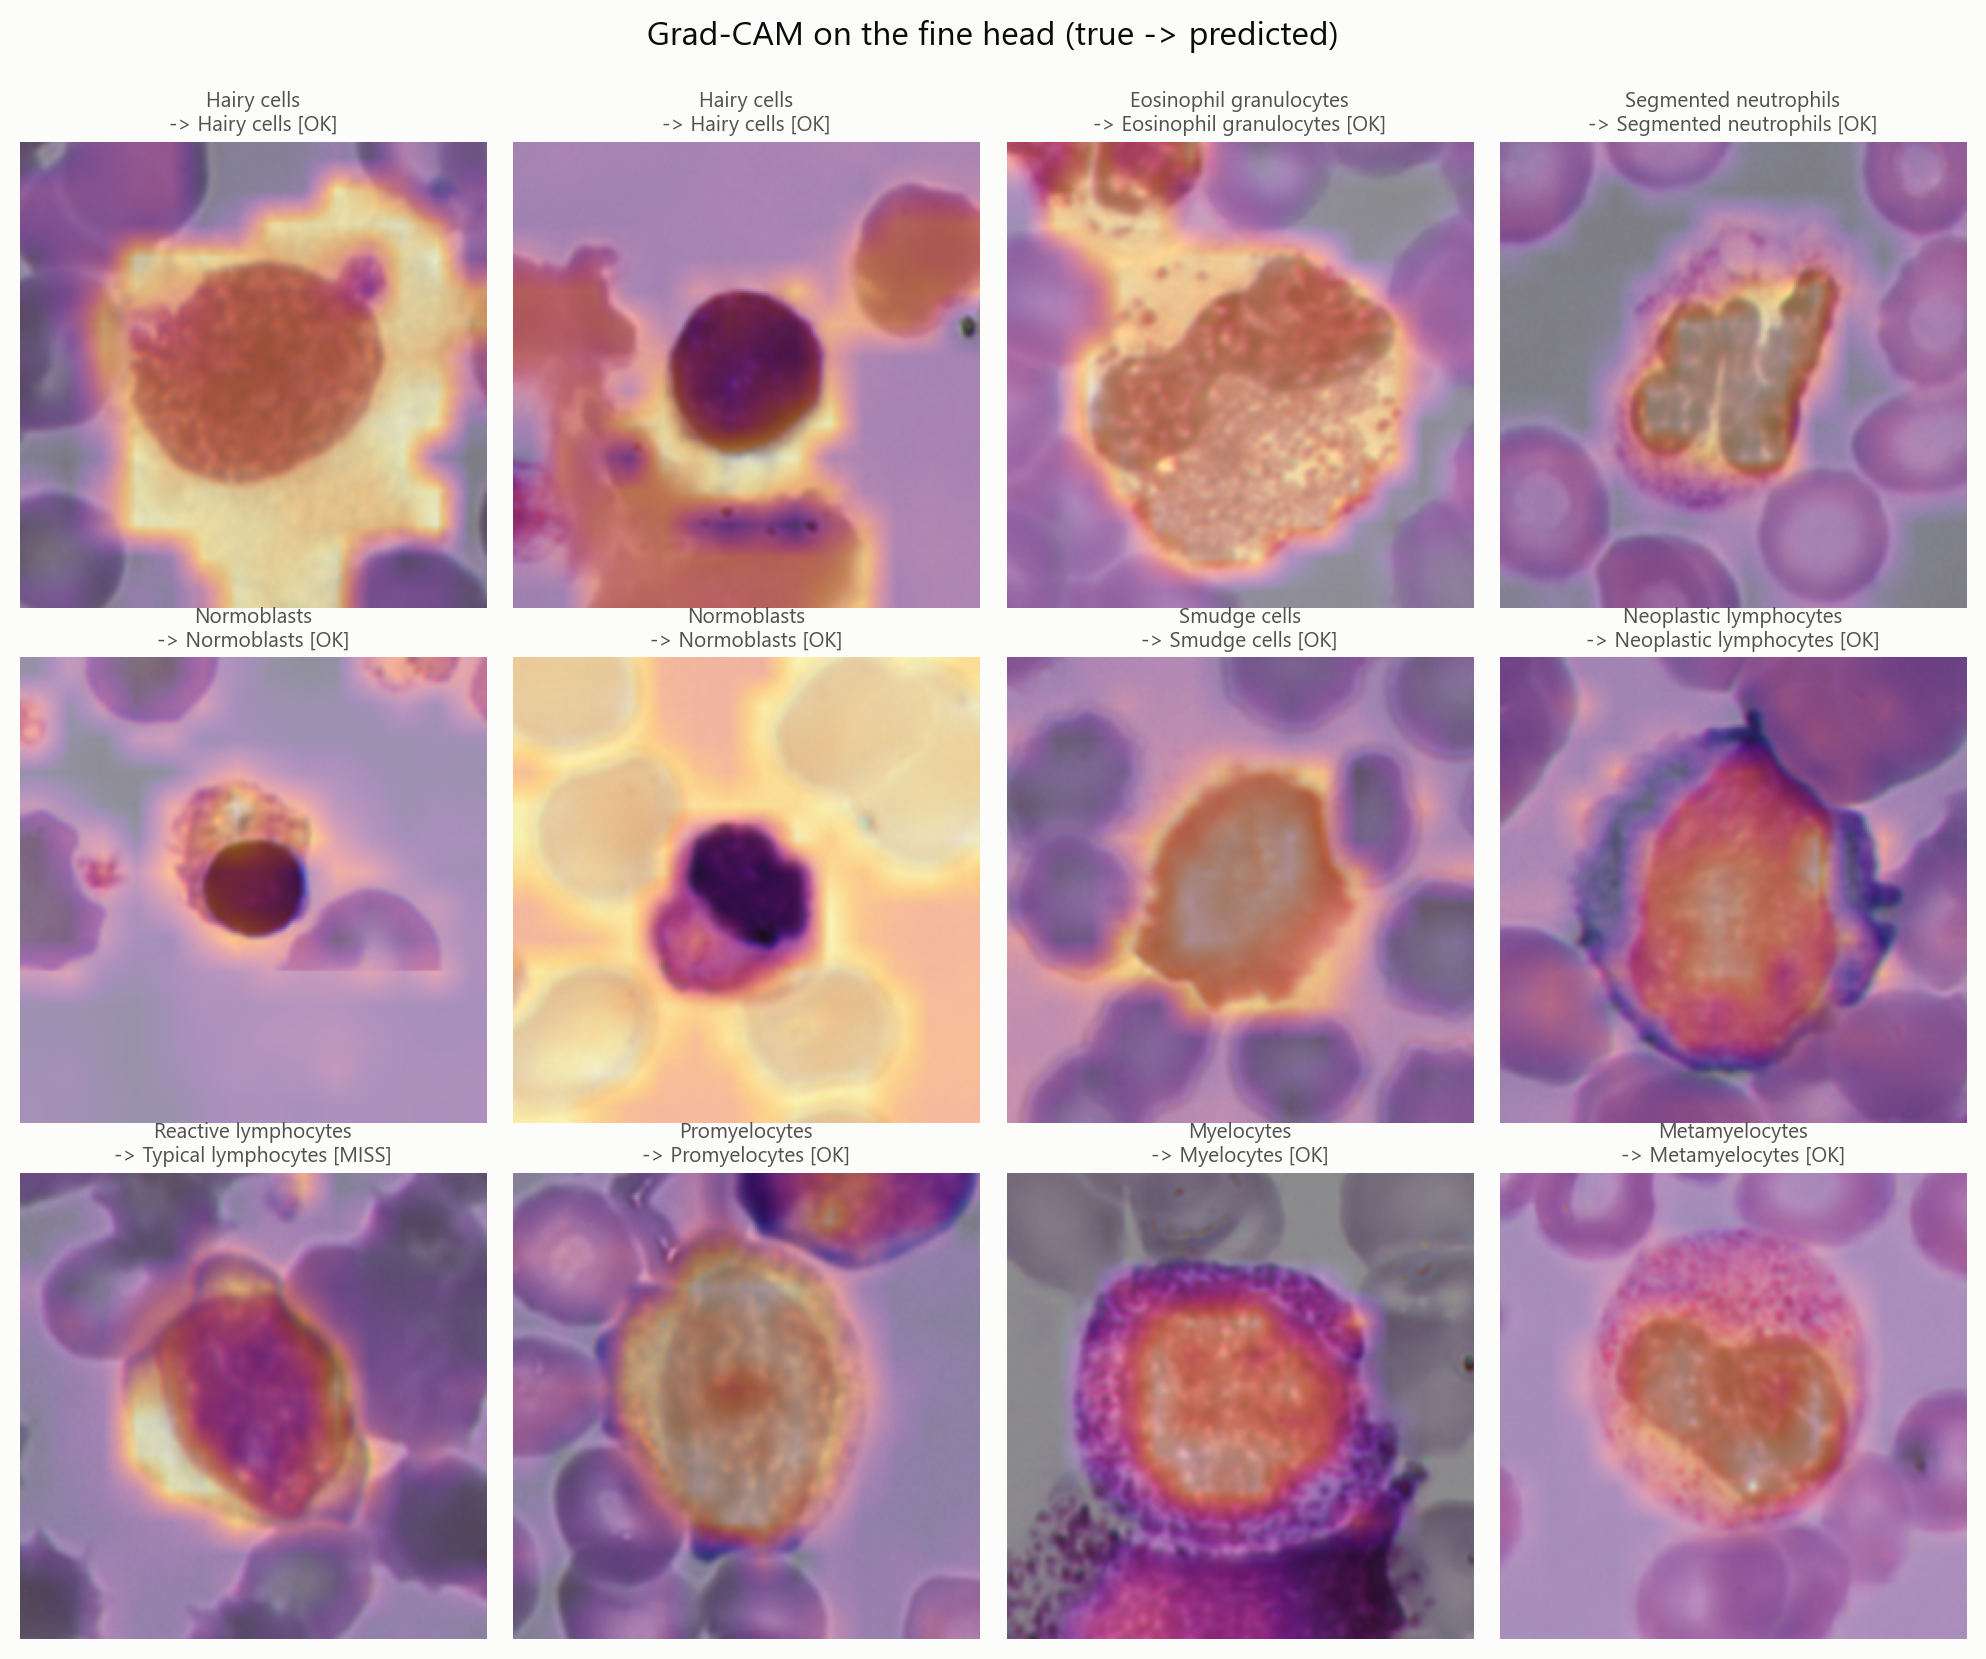
\includegraphics[width=0.82\textwidth]{gradcam_fine.png}
  \caption{Grad-CAM saliency for the fine head, with true and predicted labels.
  Attention concentrates on the cell body --- nucleus, chromatin texture and
  cytoplasmic boundary --- rather than on surrounding erythrocytes or background,
  which is the qualitative check the method is included to perform. The figure
  illustrates the technique; the saliency analysis proper belongs to the results
  chapter.}
  \label{fig:gradcam}
\end{figure}

\subsection{Statistical testing}

Because the design uses one fixed partition rather than $k$ folds, paired samples
are obtained by retraining each arm at three seeds on that fixed partition and
pairing arms by seed. This keeps the split identical across arms --- which the
ablation design depends on --- at the cost of measuring training variance rather
than data variance. For paired differences $d_i$ across $n$ seeds,

\begin{equation}
  t = \frac{\bar{d}}{s_d/\sqrt{n}},
  \qquad
  d_z = \frac{\bar{d}}{s_d}.
  \label{eq:ttest}
\end{equation}

Effect sizes are reported alongside $p$-values throughout. With three seeds the
test carries two degrees of freedom, which is thin, and reporting $d_z$ and the
per-seed values prevents the reader from being asked to lean on the $p$-value
alone.

\section{Reproducibility and threats to validity}

Determinism is enforced at three points: the partition is seeded and persisted,
each run seeds Python, NumPy and Torch from its configuration, and every
configuration is written to the results file alongside its metrics so that a
recorded run can be reconstructed exactly. Correctness is enforced by assertions
rather than by inspection --- the class hierarchy validates its own invariants at
import, downloaded counts are checked against the published figures, and the
partition is checked for empty cells, duplicates and proportion drift.

Three limitations are acknowledged. First, three seeds is a thin basis for a
paired test; it is mitigated by reporting effect sizes and per-seed values, but
not eliminated. Second, the rarest class contributes roughly 23 training images,
so its per-class F1 will be unstable across seeds; it is reported rather than
concealed inside the macro average. Third, the backbone screen uses a short
budget and selects rather than compares, so it does not license claims about the
relative merits of the four architectures.

\end{document}
